\documentclass[10pt,letterpaper,draft]{report}
\usepackage[utf8]{inputenc} \usepackage{amsmath} \usepackage{amsfonts}
\usepackage{hyperref}
\usepackage{ctable}
\usepackage{graphicx}
\usepackage{amssymb} \usepackage{ifdraft} \ifdraft {
  \usepackage[paperwidth=275.9mm, paperheight=279.4mm]{geometry}
  \setlength{\evensidemargin}{95mm}
  \usepackage[colorinlistoftodos,obeyDraft]{todonotes} } {
  \usepackage[left=1in,right=1in,top=1in,bottom=1in,paperwidth=275.9mm,
  paperheight=279.4mm]{geometry} \usepackage[obeyDraft]{todonotes} }

\usepackage[section]{placeins}
% \usepackage{minted}

\usepackage{longtable}

\author{Devin Schwab\\
  Mark Schultz\\
  David Jannotta\\
  Eddie Massey III}
\title{EECS 376/476 Mobile Robotics\\
  Team Alpha Midterm Report} \date{May 3, 2012}
\begin{document}
\bibliographystyle{IEEEtran}
\listoftodos
\maketitle

\tableofcontents
\newpage



\part{Overview}

\section{Team Members and Responsibilities}

The members of the alpha team and their respective roles are:

Devin Schwab - Group Leader, Velocity Profiler/Brushfire, A* Search

Mark Shultz - Steering, Kinect Sensor, Costmap, Brushfire

David Jannotta - Path Planning, Goal Planner

Eddie Massey III - Look Ahead, A* Search\\

In general each team member was given a specific node to work on. This allowed us to work in parallel as the interfaces to our nodes were defined prior to each node being created. However, there was some overlap between who worked on what node based on group member's expertise and availability.  For instance the Brushfire node was worked on by both Mark and Devin.

In addition to the actual coding work various other tasks were assigned. This included things like the creation of launch files, the collection of bag files and documentation.

\section{Project Goals}
The main goal for this semester was the final project. The final project involved navigating through an environment with unknown obstacles to a piece of metal, picking up the piece of metal and navigating back to the start. To accomplish this the robot needed the following capabilities:

\begin{enumerate}
     \item Take in goal destination and calculate a path to the location based on stored map information and current location
     \item Detect objects using sensors such as the Microsoft Kinect
     \item Update the overall plan as new obstacles are detected
     \item Calculate a trajectory along the desired path
\end{enumerate}

\todo[color=green,inline]{Fill out more information about each subtask}

\newpage
\section{Schedule and Milestones}

\FloatBarrier
\begin{figure}[h]
\begin{longtable}{|l|l|}
  \hline {\bf Week} & {\bf Goal} \\ \hline
Weeks 1-3 & Familiarization with ROS \\ \hline
Week 4 & Dead Reckoning Demo \\ \hline
Week 5 & Velocity Profiling Demo \\ \hline
Week 6 & Estop Demo \\ \hline
Week 7 & Obstacle Detection Demo \\ \hline
Week 8 & Steering Demo \\ \hline
Week 9 & Spring Break - Code Refactoring \\ \hline
Week 10 & Obstacle Navigation \\ \hline
Week 11 & Kinect Implementation \\ \hline
Week 12 & Farmiliarization with OpenCV and Pointcloud Library \\ \hline
Week 13 & Strap Follower Demo \\ \hline
Week 14 & Costmap Integration \\ \hline
Week 15 & Path Planning Algorithims \\ \hline
Week 16 & Integration of New Nodes \\ \hline
\end{longtable}
\end{figure}
\FloatBarrier

\section{Language Selection}

One of our biggest complaints from the first half of the semester was the fact that the C++ took so long to compile. We would spend 3 minutes waiting for our code to compile only to find that we had forgotten a semicolon on a single line. This really cut into a productivity. In addition the need to deal with memory and threading made our code difficult to write and debug.

To solve this after spring break we transitioned all of the code we possible could to python. Python takes care of memory management for us. Python's default data structures are all thread safe by default. In addition the rospy libraries take care of executing the callbacks in a separate thread. There is no need to call spin or spinOnce.

Python also solved our compilation issues.  If something was wrong we only needed to change it and save the file before running it again. We noticed no difference between the speed of our python code and our C++ code. In fact, while we have not done any real testing our code may be faster in Python simply because the underlying implementation of Python has been heavily optimized. While we believe we could have beaten Python with optimized C++ code we were not actively optimizing our code.

The only thing that could not be written in python were the Kinect nodes, the costmap node, and anything dealing with the PCL library. The Kinect node could not be written in python because the special image transport subscriber is not available in python. However, the opencv library has excellent python bindings. The costmap node could not be written in python because they don't provide wrappers. The PCL library could not be written in Python for the same reason.

We would strongly recommend advocating Python as the language of choice to future classes. The language allows one to focus more on the logic and algorithms running the robot and less on the mundane solved tasks of memory management and threading.

\section{Tools}

\subsection{Git}
\todo[color=green,inline]{Put in information about the statistics and include some of the graphs and data}
In order to keep track of the different versions of our source files
we are using git.  Our git repository can be found at
\url{https://github.com/rhololkeolke/EECS-376-Alpha}.  Using Git has
allowed us to work in parallel on the different files in our source
code and merge the various edits together.  It also has the added
benefit of keeping track of every version of our source code. There
have been many times that we have tried new changes, found they didn't
work and had to revert back to an earlier working version.

In order to keep everything organized each of us has a branch for
development.  We have also have a main branch called develop in which
we merge everyone's individual commits and do final tweaks. Every
demo is merged into master and tagged for future reference.

Git also keeps excellent statistics about who has contributed what and when code was added. See appendix A for our repositories statistics.

\subsection{ROS Launch}

Roslaunch files made splitting our packages into separate nodes easier. 
Instead of having to remember the correct executable s to run and the proper order, 
we created one launch file that incorporated each of our nodes. 
Within each node package there is a directory called launch containing its own launch file called main.launch. 
There is a launch file that finds and runs each main.launch file for each package. 
One issue that we had was the launch of the look_ahead node. In the simulator, 
look_ahead subscribes to base_scan, but on Jinx look_ahead must subscribe to the topic base_laser1_scan. 
In order to avoid having to edit and recompile our code for the module, we simply used the remap command to echo 
the subscriptions from both base_scan and base_laser1_scan. With the remap command it did not matter 
whether we were testing code on the simulator or on Jinx.

While commands from the launch files were able to assist in the versatility of our code, we did run into issues 
with launching files on Jinx. One issue was trying to use the find command to change into a package directory. The 
launch file was not able to locate the package cwru_semi_stable, so that we would be able to
 launch cwru_bringup_no_tele.launch. While the roscd command line tool was able to locate the package, 
the find function of ROS Launch XML was not capable of locating the directory. We had to work around this by 
writing a simple script to launch cwru_bringup_no_tele.launch and start_amcl_2ndfloor.launch.
While ROS Launch XML is a great framework there could be better documentation and high consistency for ease of use.



\subsection{Unit Testing}

Because of the complexity of each node and the system as a whole it can be extremely difficult to debug. The best practice is to prevent bugs from manifesting in the first place. Unit testing is an approach to help catch bugs before they become lost in the system. It involves writing a suite of automated tests for each function in the nodes. In general it is best to write the tests before the actual code is written as this forces the developer to think through all of the implementation decisions before writing any code. However, due to the highly dynamic nature of our code base and the compressed time in which we had to do demos we do not have a comprehensive unit testing suite.

Also, while unit testing is an excellent tool to catch bugs before they happen and prevent regressions in functionality it should be noted that they are not fool proof.  For instance the unit tests will not cover every case, and so it is possible that edge case bugs can still slip through into the final project. In addition if the unit tests have bugs then the functionality of the code it is testing cannot be properly evaluated. However, most tests are quite simple compared to the actual code implementation and so bugs that do appear in the test are usually far easier to catch than those that are in the real software.

In our project we used two unit testing frameworks: GTest and PyTest

\subsubsection{GTest}

GTest is Google's C++ Unit testing
framework.\cite{google_googletest} ROS recommends
its use for unit testing needs. At the beginning of the semester we were using it to test 
helper classes, but after the switch to python we did not use it as much. However, it would still have been useful for the nodes that dealt with the Kinect as we could not use python for those modules.

\subsubsection{PyTest}

PyTest is included with standard python distributions so it is easy to set up and run a test on any computer with python.  Python is easier to do unit testing with because of duck typing.  Duck typing refers to the phrase, ``If it looks like a duck and quacks like a duck, it must be a duck.'' \cite{python_duck_typing} This refers to python's weak typing. In strongly typed languages such as C++ in order for a method to accept a parameter it must be the type defined in the function. In python the type doesn't matter, the only thing that matters is if the parameter implements the methods that are called on the parameter. This means multiple classes can be passed into a single method as long as they all implement the same methods. This is similar to Java's interface concept, except the interfaces do not need to be explicitly specified.

The reason duck typing is useful is that we can easily write small prototyping classes for our own classes and for ROS classes. These classes can provide a very limited simulation of what the real class would provide. This means that even functions which depend on things which are difficult to control , such as network communications, can be tested by writing a mockup class.

\subsection{Integration Testing}

While Unit testing works great for functions and small pieces of classes and nodes, it does not necessarily lend itself to testing the integration of multiple nodes. Especially when the other nodes have not been implemented yet. Also the unit testing is not easily used with the simulator. Additionally, certain tests can only be run in the simulator.

To get around this problem we created small prototype nodes that would take in user input either from the command line or csv files and interact with the other nodes based on this. For instance to test the velocity profiler class a path publisher prototype was created. This prototype took in a csv file that specified a list of path segments and it published them using the PathList message. This allowed velocity profiler to be tested before the nodes on the other side of the interface were actually completed.

Our integration tests are contained in folders called integrationTests within each node's package.

\part{Software Architecture}

Before writing the code for the demos, we started by coming up with an
overall software architecture.  The purpose of this planning was to
write each node so that as other nodes are added to our software
package we do not have to spend time rewriting old code.

This section will describe the decisions we made and what we have
planned.

\section{Node Architecture}

The main document we are basing our software architecture off of is
the following:

\FloatBarrier
\missingfigure{Attach the updated software architecture drawing}
\FloatBarrier


This figure clearly shows the different nodes we have planned, the
communication message types being passed between them, and areas of
possible future expansion.

The specifications for the nodes in the diagram and the messages being
used will be found in the rest of this section.

\section{ROS Packaging and Stacks}

We have been utilizing ROS stacks to manage our individual ROS packages.
We will try to use a single package per node. This will encourage
appropriate message passing between nodes and make sure they are not too
tightly coupled.

Another benefit is that rosmake will build packages that don't depend
on one another in parallel.  This decreases the build time by a small
amount, which is especially useful when making small changes during testing.

Stacks utilize a \texttt{stack.xml} file which contains dependencies to
be included for every package. The ROS stack will automatically build
all packages within it's root directory.

Complete documentation can be found at 
\url{http://www.ros.org/wiki/Stacks}


\section{Node Specifications}

To help guide us while writing our nodes we wrote a small
specification for each class seen in the software architecture diagram.

\subsection{Velocity Profiler}
This nodes is responsible for taking in a list of path segments through the PathList and PathSegment message. After receiving the specified path, velocity profiler calculates the optimum trajectory based on the velocity and acceleration constraints in specified in the path segments. In the process of computing the optimum trajectory velocity profiler will blend multiple segments into a single seamless trajectory. After the trajectory is computed velocity profiler is responsible for sending the desired velocity at each point to steering.

\subsubsection{Requirements}
\begin{enumerate}
  \item Velocity Profiler must accept PathList messages
  \item Velocity Profiler must calculate spatial trajectories from
        the accepted PathSegment messages
        \begin{enumerate}
           \item Velocity Profiler must obey all of the path constraints
                 specified in every accepted PathSegment message
        \end {enumerate}
  \item Velocity Profiler must respond to Obstacle messages from Look
        Ahead
        \begin{enumerate}
           \item Velocity Profiler must stop and wait at an obstacle for a
                 specified amount of time
           \item Velocity Profiler must alert Path Planner if an obstacle
                 has not moved after a specified time
        \end{enumerate}
   \item Velocity Profiler must publish a desired velocity based on the computed trajectory
   \item Velocity Profiler must stop when the E-Stop is enabled
   \item Velocity Profiler must resume a plan after the E-Stop is
         disabled
\end{enumerate}
      
\subsection{Look Ahead}

This node enables reactive obstacle detection. As the name implies it is responsible for ``looking'' ahead for obstacles along the path. Currently it uses the LIDAR but using either the costmap or custom code this could be expanded for other sensors such as the Kinect.

  \subsubsection{Requirements}
  \begin{enumerate}
     \item Look Ahead will parse the data from the LIDAR
     \item Look Ahead will detect objects within a minimum of 1 m along the specified path
     \item Look Ahead will exclude obstacle detection of all objects
           outside of the planned path
  \end{enumerate}

\subsection{Steering}
  This node is responsible for correcting the small differences
  between desired and actual heading. It takes in a desired velocity and scales
  its own steering around that value based on the segment type.

  \subsubsection{Requirements}
  \begin{enumerate}
     \item Steering will accept a list of paths
     \item Steering will correct the desired velocities from Velocity
           Profiler
     \item Steering will obey stopping commands in the desired velocity
     \item Steering will stop correcting the path when the E-Stop is pressed.
  \end{enumerate}

\subsection{Path Planner}

This node is responsible for taking in a set of path points and converting it to a list of path segments that form a path through the desired points. It is allowed to throw out conflicting data and select path segment parameters such as the speed.

  \subsubsection{Requirements}
  \begin{enumerate}
    \item Path Planner will receive a list of path points
    \item Path Planner will send out the calculated path in segments
    \item Path Planner will respond to requests for new paths
    \item Path Planner will correct its computed path based on new information in the path point list
  \end{enumerate}

\subsection{Path Finder}

This node is responsible for taking in sensor information and map information and finding a potential points that the robot should navigate to. These points will eventually be constructed into a path segment which will be put together to make an entire path. We implemented multiple instances of this node.

     \subsubsection{Requirments}
     \begin{enumerate}
       \item The path finder will not suggest points in which an obstacle is known to exist
       \item The path finder will return the points in the order in which it suggests navigating to
             them
       \item The path finder will update its suggestion over time as new information is provided
     \end{enumerate}
 
\subsection{Kinect}

This node is responsible for any vision processing and depth map processing that the other nodes need to accomplish their goals.  This includes things such as color detection (based on the image data) and distance detection (based on the depth map). Multiple binaries are included in this node. Each accomplishes different things. The launch file can be customized to launch the ones that are necessary for the task at hand.

  \subsubsection{Requirments}
  \begin{enumerate}
    \item The Kinect node shall receive information from the Microsoft Kinect sensor
    \item The Kinect node shall provide the image processing capabilities to any node that desires it
    \item The Kinect node shall provide depth information to any node that desires it.
  \end{enumerate}

\subsection{Costmap}

This node is responsible for populating the robot's representation of the world map with places it cannot go. It will do so using information from the sensors.

  \subsubsection{Requirments}
  \begin{enumerate}
    \item Costmap shall receive information from the different sensors on the robot
    \item Costmap shall provide a list of points which the robot cannot visit.
  \end{enumerate}
       
\subsection{Goal Planner}

This node is responsible for commanding the movement nodes in order to accomplish useful tasks. This node operates at a higher level from the other nodes and is not concerned with how the robot goes places, only that it goes to the places that goal planner commanded it to go to. Goal planner can receive sensory information in order to determine the places the robot should be going.

  \subsubsection{Requirements}
  \begin{enumerate}
    \item Goal planner shall be capable of determining where the robot should go to accomplish its tasks
    \item Goal planner shall give the movement nodes waypoints to navigate to
  \end{enumerate}

\todo[color=red,inline]{Check the definitions of new message specifications.}
\section{Custom Message Specifications}

\subsection{SegStatus}

Responsible for holding information about the status of a path
segment.  The message format is as follows:

\noindent {\bf uint64 lastSegComplete}\\
\indent Stores the number of the last segment that was fully executed.\\
\\
{\bf uint64 seg\_number}\\
\indent Stores the number identifying the segment the message is
pertaining to.\\
\\
{\bf float64 distance}\\
\indent Stores the distance remaining on a segment.\\

\subsection{Obstacle}

Responsible for holding information about obstacles in the path
segments.  The message format is as follows:

\noindent {\bf bool exists}\\
\indent True when 1 or more obstacles detected in path\\
\indent False when 0 obstacles are detected in path\\
\\
{\bf float64 distance}\\
\indent The distance to the closest obstacle\\

\subsection{BlobDistance}
The Kinect Listener publishes the distance from the center of an image
to the center of a blob.

\noindent {\bf uint32 dist}\\
\indent Distance from the center of the blob to the center of the vision in pixels\\

\subsection{CentroidPoint}
Contains the centroid of the interesting part of an image.

\noindent {\bf bool exists}\\
\indent True when a centroid is found (i.e. image filtering criteria is met)\\
\indent False when no interesting parts are left in the image after filtering\\
\\
\noindent {\bf geometry\_msgs/Point point}\\
\indent The point at which the centroid is.\\

\subsection{Goal}
Incrementally updates the major waypoints the robot is supposed to reach.

\noindent{\bf bool new}\\
\indent True when a new goal is published.\\
\\
\noindent{\bf bool none}\\
\indent Set to true when the robot should not change its present location.\\
\\
\noindent{\bf geometry\_msgs/Point goal}\\
\indent The coordinates of the desired goal\\

\subsection{PathList}
A list of path segments that make up a path.

\noindent {\bf msg\_alpha/PathSegment[] segments}\\
\indent The path segment specifications that the robot must follow, in the order they must be followed.\\

\subsection{PathSegment}
Path Segments that are generated by the Path Planner node.

\noindent {\bf int8 seg\_type}\\
\indent The segment type can be a line, arc, or spin, 1,2 or 3 respectively.\\
\\
\noindent {\bf bool relative}\\
\indent Set to true when the path is in the robot's coordinate frame.\\
\indent Set to false when the path is in the map's coordinate frame.\\
\\
\noindent{\bf float64 seg\_length}\\
\indent The length of a path segment.\\
\\
\noindent{\bf geometry\_msgs/Point ref\_point}\\
\indent The reference point of a path segment.\\
\\
\noindent{\bf geometry\_msgs/Quaternion init\_tan\_angle}\\
\indent The initial tangent angle of a path segment.\\
\\
\noindent{\bf float64 curvature}\\
\indent The curvature of a path segment.\\
\\
\noindent{\bf geometry\_msgs/Twist max\_speeds}\\
\indent Maximum speed for a path segment.\\
\\
\noindent{\bf geometry\_msgs/Twist min\_speeds}\\
\indent Minimum speed for a path segment.\\
\\
\noindent{\bf float64 accel\_limit}\\
\indent Acceleration limit for a path segment \\
\\
\noindent{\bf float64 decel\_limit}\\
\indent Deceleration limit for this segment.\\

\subsection{PointList}
Points that the robot should be steering to.

\noindent{\bf bool new}\\
\indent Set to true if points in the message have changed\\

\noindent{\bf geometry\_msgs/Point[] points}\\
\indent Contains the list of points in the order they are supposed to be used in\\

\section{Topics}

\subsection{des\_vel}
Velocity Profiler publishes the desired velocity based on the robot's
current point in space the current and next path segments.  This
velocity is then corrected by steering.

\subsection{cmd\_vel}
Steering publishes the final velocity to the robot's motors.  The
final velocity is a corrected version of the velocity in the des\_vel topic.

\subsection{base\_laser1\_scan and base\_scan}
base\_laser1\_scan is used on the robot\\
base\_scan is used in the simulator\\

\noindent Used to send out LIDAR data from the cRIO.

\subsection{seg\_status}
Velocity profiler publishes the status of its current segment on this
topic.  Nodes such as steering subscribe to it.

\todo[inline]{Check over descriptions}

\subsection{path\_seg}
Path Publisher publishes the planned path segments to this topic.  The
published segments are used by steering, velocity\_profiler and other nodes.

\subsection{point\_list}
AStar publishes a list of points for the pathplanner to generate path segments from.
\subsection{goal\_point}
The goal publisher sends a goal to the AStar node that determines the end point of the A star search.
\subsection{path}
The path list determiend by the path planner.
\subsection{obstacles}
Look ahead publishes whether or not there is an obstacle within the bounded box area directly in front of the robot.
\subsection{motors\_enabled}
Estop publishes whether or not the estop is off.


\part{Nodes}
\todo[inline]{Each person will write this section based on the one you
  have worked on}
In the software architecture section the specifications for each node
was discussed.  This section deals with the actual implementation of
each node.  This includes problems encountered, solutions found, and
future plans

\section{Velocity Profiler}

\subsection{Theory of Operation}

Velocity Profiler is responsible for generating a trajectory from the path segments provided by Path Planner.  Velocity Profiler is also responsible for keeping track of where the robot is in the computed trajectory. It provides the desired velocity based on the current desired trajectory to steering which then adds correction factors before it is finally sent to the robot's motors.

There were two methods of generating the trajectory, time based and
spatial based.  We chose to implement the spatially based method
because it made it easier to stop and resume the robot due to E-Stops
and obstacles in the path.

\subsubsection{Velocity Profiling Algorithm}

The current version of velocity profiler takes in segments published by the Path Planner in the form of a PathList message. This PathList message contains PathSegment specifications which give the position in space of path in small chunks. PathSegment messages also contain information about the constraints on that section of the path. Velocity profiler uses these constraints to compute things like the point in space to start and stop accelerating.

Each time a list of path segments is received, velocity profiler checks for changes in the segment number. Velocity profiler works under the assumption that the segment number is a unique id for a segment and that segment numbers will not decrease except in the event that a path is aborted. If a single segment has been changed then velocity profiler will recompute the trajectory. It would be difficult to recompute the trajectory for only the part that has changed because more segments then the ones that have changed can be affected by a change in a single segment. For instance if the minimum speed in a segment is raised it may mean that the next segment will need to immediately begin braking whereas before it may have accelerated. To avoid having to propagate effects of a single segment change throughout the entire trajectory velocity profiler simply starts from scratch each time it receives a segment.

In order to blend segments velocity profiler keeps track of the starting and ending velocity of each segment. Transitions between spin segments and lines and arcs require a full stop, but transitions between lines and lines, arcs and arcs, and arcs and lines can be blended together so that the robot may slow down, but it will not come to a complete halt.

Because of the structure of the velocity commands straight and spin commands can be profiled separately and each component can be controlled by velocity profiler to execute complex maneuvers. Arcs require that the spin trajectory be constrained to the speeds of the straight trajectory.

Velocity profiler uses an internal class called TrajSeg.  This class stores information about a single segment in the trajectory and provides a reference to the pathsegment instance to which it corresponds. This segment contains the type -- acceleration, deceleration, or constant velocity -- was well as stopping distance in terms of normalized segment length and start and stop velocities.  Using this information the velocity controller can execute a trajectory simply by looking at the next trajectory segment and using the information in it until its reached a point past the trajetory segment's stopping point.

To compute the trajectory segments the following basic kinematic equation is used:
\begin{center}
$v_f^2 = v_i^2 + 2*accel*dist$
\end{center}
Using this equation in the forward direction from the beginning of the segment velocity profiler can determine the stopping point of the acceleration portion of a path segment (if there is one). Using the equation in reverse starting from the end of the path, velocity profiler can determine the starting point of a deceleration segment and consequently the stopping point of a constant velocity segment.  If the starting point of the deceleration segment is before the stopping point of the acceleration segment there will be no constant velocity segment.

When calculating the acceleration stopping point if the result is negative then it means the final speed of the previous segment is faster than the maximum speed of the current segment and so the robot must actually start with a deceleration segment. Ideally this will never happen, however, it is difficult to check for this condition and its importance was not deemed high enough to justify the computation time. A similar thing can happen with the deceleration segment if the number comes out greater than 1.0 (the normalized path length). In that case the robot shouldn't decelerate, but neither can it accelerate without violating its maximum velocity constraint. In that case there will be no deceleration segment.

\subsubsection{State Class}
Velocity Profiler uses an internal class called State.  This class is
responsible for figuring out how far along the path the robot has
traveled.  This is used to determine when a segment is completed and
the next one should be loaded.

The first version simply integrated the velocity commands over time to
keep an internal belief state of where it is at. This caused problems because steering modified the velocity commands which made the internal belief state fall out of sync with reality.  To fix this we originally fed back in the steering commands that were actually sent to the robot. However, it was difficult to use. Instead because map position data is already available and the trajectory is already specified in terms of space points an entirely different algorithm was developed based on the geometry of the path segments.  Because each of the three segment types has a unique geometry each type of segment is dealt with differently.

\paragraph{Line Segments}
The lines work by assuming that the path segment is actually an infinitely long line. It then takes the robot's position and finds the line passing through this point and normal to the path segment line. The intersection of this line with the path segment line is found. The intersection points distance from the starting point of the path segment is then computed. Using the tangent angle of the path segment the state class determines if the point is before or after the starting point on the hypothetical line.  If the intersection point is before then the segment distance completed is negative otherwise it is positive. Also the segment distance completed is normalized with respect to path length meaning that numbers between 0.0 and 1.0 are within the specified path segment, numbers greater than 1.0 are past the end of the segment and numbers less than 0.0 are before the start of the segment.

\paragraph{Spin Segments}
The spins simply uses the orientation of the robot. The state class turns the initial tangent angle of the spin into a number between 0 and $2\pi$. It does the same for the orientation data. It then takes the difference between the current angle and the desired angle.  If the angle is positive then it will give a segment distance done greater than 0.0 and otherwise the number will be less than 0. There are some issues with wrap around on the unit circle.  To handle this I make sure all of the angles are referenced with respect to the 0 angle. Having a common reference means that I can tell where each angle is in relation to each other by referencing it with respect to the common reference. From there I transform the angles into a reference based on the initial tangent angle. This allows me to ignore wrap around of $2\pi$ to 0 on the unit circle.

There is a slight problem with this approach for the spins. Because of the wrap around it is necessary to specify a specific angle that will transition the segment distances done from negative to positives. To do this an angle halfway between the start and final angle of the spin segment is computed and $\pi$ is added to it. The problem with this approach is that the longer the spin in terms of radians the more likely it is the robot will skip over a number greater than 1.0 and cycle back around to a negative number. Also spins longer than $2\pi$ cannot be specified. This was not a real problem because we can split long segments into smaller ones and velocity profiler will blend them together.

\paragraph{Arc Segments}
The arcs are the most complicated, but share many similarities with the spin computations. The main difference is that the spins cannot have an offset from the center of the circle whereas the arcs can. For the arcs I start by finding the angle of the line from the robots current position to the specified arc's reference point. Originally the algorithm planned on looking for the intersection of this line segment with the circle that the arc would make were it long enough. However, the formula was difficult to compute and it was difficult to translate that point to a segment distance complete number like in the lines and spins algorithm. After finding the angle of the line between the robot and the arc's center all of the angles are converted to numbers between 0 and $2\pi$. This ensures that all the angles are referenced to the 0 angle making it far easier to compare where on the circle each angle is. The rest of the angle computations are the same as for the spin segment.

In order to test this algorithm a number of matlab scripts that plot the results of these calculations were written. These scripts made it easy to visualize the outcome of the computations and to see how the different parameters affected the outcome. An example image output is shown in figure ~\ref{fig:arcComputationExample}. In the figure the solid blue line is the specified arc segment, the dashed blue lines are the starting and final angles. The red dot on the blue line is the starting point. The magenta dot-dash line is the cutoff angle between negative and positive angles. The magenta x is the robot's position. The green dashed line is the line from the robot to the arc's reference point. The black x is the point on the circle that the line from the robot to the arc's reference point intersects the circle that a complete arc would specify.

\FloatBarrier

\begin{figure}[h]

  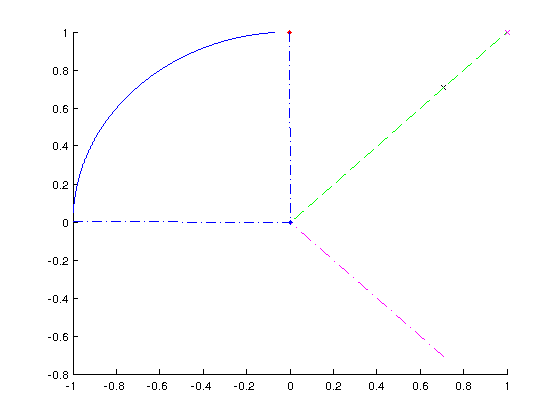
\includegraphics{images/arcComputationExample1.png}
  \caption{Robot at position (1,1,0) for an arc with curvature of 1.0, length of pi/2, starting angle of pi/2 and a center at (0,0,0). The segment distance completed is -0.5}
  \label{fig:arcComputationExample}
  
\end{figure}

\FloatBarrier

The code used to generate this figure is included in the report, but you can view the repository at \url{https://github.com/rhololkeolke/Velocity-Profiler-Simulations/}

\subsection{Observations}

Keeping track of segment completion the way velocity profile does allows our path planner to be a little sloppy in the path segments its publishing. The path segments don't have to start exactly where the robot is at and there can be small gaps and offsets between the different path segments. Steering will correct any path offsets and orientation errors and the velocity profiler will simply keep track of how close it is to the end along the specified segment.

As mentioned in the algorithm description having a hard cutoff between negative and positive segment distance done values for arcs and spins can cause problems for long segments. One way to solve this is to use short segments like we did. Another way is to combine the original integration algorithm with our current algorithm. At the beginning of the algorithm the integration data is really accurate, however, as the robot moves the integration data gets less and less error. To account for this each algorithm could be used in something like a Kalman filter or particle filter. At the beginning of the segment the ``believability'' of the integration will be very high and will dominate, as the robot moves this believability will decay and eventually the new algorithm will dominate.

\documentclass{article}
\usepackage{graphicx}
\begin{document}

\section{Look Ahead}
\subsection{Theory of Operation}
The look ahead node is responsible for obstacle detection. The node subscribes
to lidar data to and uses trigonometric functions create a configuration space
that resembles a bounded box. The configuration space is determined by creat-
ing a box of lidar pings slightly larger than the perimeter of the robot (1m by
0.5m). The C-Space is directly in front of the robot. Below is a list of Constants
used in the look ahead source file:\\
const uint cPings = 181; The data from the laser comes from the topic sensor$\textunderscore$msgs$\backslash$LaserScan
and is passed into an array large enough to hold 181 values (one for each ping)\\
const double cBoxHeight = 1.0; This value corresponds to the height of the\\
c-space bounded box
const double cBoxWidth = 0.5; This value corresponds to the width of the
c-space bounded box
The node constantly publishes to a custom message type called “obstacles.”
If an obstacle is found within the configuration space then the look ahead node
publishes true (an obstacle exists) and the obstacle’s distance along the current
path, otherwise the node publishes false for the obstacles existence and 0 for its
distance. Obstacle detection is mathematically derived. If a lidar ping returns
and it is less than the height or width of the c-space divided by cos$\theta$ where $\theta$ is
in radians then an obstacle exists.\\\\

$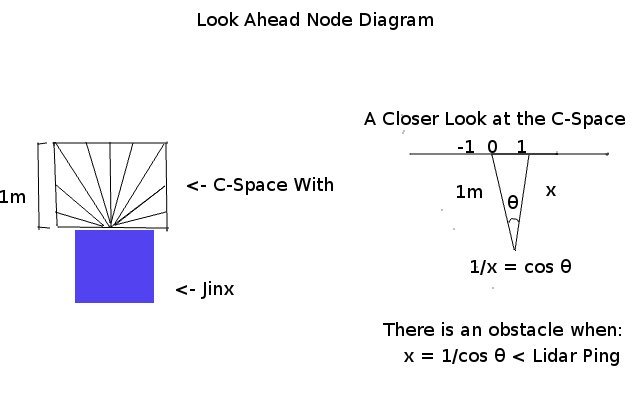
\includegraphics[scale = 0.5]{look_ahead.jpg}$ \\
Figure 1 - Represented by lines 56 - 77

Figure 1 is reproduced in our code through this example:\\\\
\indent if(curLaserData[i] $<$ cBoxWidth/cos((180.0-(double)i)*M PI/180.0))\\
\indent \indent$\{$\\
\indent \indent \indent if(curLaserData[i] $<$ closestObs)\\
\indent \indent \indent$\{$\\
\indent \indent closestObs = curLaserData[i];\\
\indent \indent \indent$\}$\\
\indent \indent$\}$\\
The above code snippet means that if the lidar ping is less than the width of the bounded box divided by cos$\theta$ an obstacle exists and its distance is the distance the lidar ping returns.\\

After the algorithim was properly developed one inital problem with the look ahead code was the lidars 80m
range. In order to make sure that lidar data was not misinterpreted beyond
the bounds of the box we created a value of closestObs and set it to 90(m).
Since the lidars range is 80 there shoudld definetley not be any object detected
beyond the length of closestObs.

\subsection{Observations}
Lidar detection obstacle detection is not good while turning. There seems to be
a blind spot right next to the lidar scanner.

\subsection{Future Plans}
Presently our c-space configuration algorithim will not suffice for arced paths. We plan on doing some modifications to the look ahead source code to ensure the robots ability to detect obstacles at any given instance. The node will aslo need to receive segment status messages to determine if there is an obstacle path on the type of path the robot is considering moving along.

\end{document}






\missingfigure{Attach an image of the derivation of the geometry for
  the look ahead box}

\section{Steering Node}

The Steering node is responsible for taking the desired velocities from
the velocity planner, the desired path from the path planner, and the
current position to determine correction factors to the velocity command
such that the robot does not stray from its desired path.

\subsection{Theory of Operation}

We use a number of messages to control the steering node.

\begin{itemize}
\item
  Path segment: the path segment node passes in the current path segment
  we would like the steering node to follow.
\item
  vel\_des: this message gives us the desired velocity as determined by
  the velocity\_profiler.
\item
  TODO: others?
\end{itemize}
\subsubsection{Steering Algorithm}

We will use the linear steering algorithm. This algorithm takes a number
of inputs such as:

\begin{itemize}
\item
  The $x$ and $y$ coordinates of the destination.
\item
  The current $x$ and $y$ coordinates.
\item
  Tuning parameters $K_d$ and $K_\theta$
\end{itemize}
First we use the path segment coordinates to calculate the desired
heading with the following: $atan(yf-ys,xf-xs)$. Next we find a
$d_\theta$ by subtracting $heading_{dest}-heading_{curr}$. We can
prevent turning the long way by checking to see that $d_\theta$ is less
than or greater than $\pi$. Finally, we take the vector components of
the desired heading $tx=cos(heading_{dest})$, $ty=-sin(heading_{dest})$
and dot these with the vectors from the start point to the current point
$xrs*nx+yrs*ny$. We take this product and add it to $d_\theta$ to get
the final corrected heading $-K_d*offset+K_{\theta}*d_\theta$.

\subsection{Observations}

We ran into several problems when trying to perfect our steering code.
The hardest part of this demo was getting all of the previous nodes
integrated and functioning. We had to integrate several dummy messages
and structures to glue together everything until all the nodes can be
completed.

-TODO: describe bug where the robot would get too close to the door on
the first turn

\subsection{Coding Procedure}

The \texttt{steering\_example.cpp} sample code was tweaked to include a
file reader to allow us to easily modify constants $K_d$ and $K_\theta$.
We also ended up coding a rudimentary path planner that has hard coded
path segments.

\subsection{Future Plans}

\begin{itemize}
\item
  Non-linear steering: We plan on replacing the linear steering
  algorithm with the non-linear one
\item
  Arc path steering: We plan on generating arch path segments and
  allowing the steering node to maintain control over these segments.
\item
  Python source code: We plan on porting all of our existing code to
  python. We would like to utilize rospy for ease of programming and to
  get rid of compile time.
\end{itemize}


\todo[inline]{Fill in new node information}

\section{Pathplanner Node}

The path planner subscribes to the message published by the astar or the brushfire nodes, depending on which is in use at the time. The node then determines a series of short paths and publishes a list of them.

\subsubsection{Path Planning Algorithm}
The algorith takes in the points published by the astar and brushfire nodes. Using these points, it calculates both the length and heading of the individual segments.

\subsection{Implementation}


\subsection{Observations}


\subsection{Future Plans}
One of the main flaws of the current path planner is that given points with enough space between them, it will ultimately propduce an uneven, rough path. This is primarily because the current point publishing node publishes a list of points which are very close together. This issue can be solved with the use of a smoothing algorithm. In the next itteration of the code, this will be implemented.


\section{Position Publisher Node}

What do I do?

\subsection{Theory of Operation}


\subsubsection{Position Publisher Algorithm}
 This algorithm takes a number
of inputs such as:


\begin{itemize}
\item
  stuff
\item
  stuff
\item
  stuff
\end{itemize}


\subsection{Implementation}


\subsection{Observations}


\subsection{Future Plans}

\begin{itemize}
\item
  stuff
\item
  stuff
\item
  stuff
\end{itemize}


\section{Costmap}

What do I do?

\subsection{Theory of Operation}


\subsubsection{Costmap Algorithm}

 This algorithm takes a number
of inputs such as:

\begin{itemize}
\item
  stuff
\item
  stuff
\item
  stuff
\end{itemize}


\subsection{Implementation}


\subsection{Observations}


\subsection{Future Plans}

\begin{itemize}
\item
  stuff
\item
  stuff
\item
  stuff
\end{itemize}


\section{Goal Planner Node}

What do I do?

\subsection{Theory of Operation}


\subsubsection{Goal Planning Algorithm}
 This algorithm takes a number
of inputs such as:


\begin{itemize}
\item
  stuff
\item
  stuff
\item
  stuff
\end{itemize}


\subsection{Implementation}


\subsection{Observations}


\subsection{Observations}


\subsection{Future Plans}

\begin{itemize}
\item
  stuff
\item
  stuff
\item
  stuff
\end{itemize}


\section{Kinect Node}

The Kinect node contains 2 main programs. A blob finder used in the first Kinect demo and the strap following code that was used in the strap following demo.

\subsection{Theory of Operation}

The Kinect node contains multiple discreet binaries that the other nodes can start up and receive information from if needed. We did this because it made sense to group all of the Kinect code in a single place, yet it also made sense to make separate executables for the wide range of vision applications available.

\subsubsection{Kinect Algorithm}

The blob finder used only image data. OpenCV was used to process the received image data. The blob finder started by converting the received image into a binary image based on the RGB thresholds set in the launch file. Then we eroded the image and dilated what was left. We then ran a segmentation and blob detection algorithm on the filtered image. From the detected blobs we selected the largest and published its centroid in terms of image pixels from the center in the horizontal direction.

The strap follower was more sophisticated then the blob follower. It filtered the image in a manner similar to the blob finder, however, it used HSV values instead of RGB values. It also utilized the depth map information. After filtering on color it took the remaining pixels and transformed their image coordinates into base\_link coordinates. If the coordinate was within certain z-thresholds it was ignored. The points that were within the z-thresholds were put into a grid. The grid can be thought of as similar to a 2D histogram. Each cell in the grid is a bin and points within the cell's bounds all get put in that same bin.

After the points were classified in the bin the centroid of each bin was calculated. Those bins with no points in it were ignored. The bin with the closest centroid was remembered and that point was published as the next point in the strap to go to.

\subsection{Implementation}
The blob finder actually used the older C openCV libraries. These were much harder to use and it took some time to figure out how to get the CMakeList to properly link all of the files. For the strap follower we made sure to use the new up-to-date C++ libraries.

Instead of the bin algorithm we originally tried to use some of the new features of the Point Cloud Library (PCL) such as voxels and octrees.  However, we could not get these to compile on the robot because of an older version of the PCL that did not have the methods we needed.

We also tried using the filter functions of the PCL library but could not figure out how to get it to compile because it used Boost pointers which do not act the same as a standard C++ pointer.

\subsection{Observations}

The blob finder had a lot of noise. We believe we should have averaged the centroids over time. In addition we had problems with using RGB for filtering. The night before the demo we had it working, but when it came time to do the demo because of slightly different lighting conditions we could not consistently pick up the strap. Luckily we had our threshold values in specified as parameters in the launch file so it was easy to change on the file.



\section{Astar Node}

The Astar node is responsible for generating the most optimal path given a list of closed points from a rolling costmap and a goal from the goal publisher.

\subsection{Theory of Operation}
After a costmap is generated it publishes to the topic inflated\_obstacles. The Astar node listens to that topic and converts each obstacle's map position into the node's own grid frame. AStar also listens to the goal\_point topic to find out the desired destination in map coordinates. The goal point is also converted to the node's grid frame. The node takes the obstacle points and adds them to a closed list. From the closed list the Astar node is able to generate the most optimal path to the goal point.


\subsubsection{AStar Algorithm}
The robot's starting position is added to the open list. The neighboring location on the map with the lowest F is added to the open list and then switched to the closed list. For each adjacent location:

\begin{itemize} 
\item If the space is an obstacle or on the closed list ignore it.
\item If it is not on the open list add it to the open list. Make the current square the parent of the square and update the cost, heuristic, and sum of the cost and heuristic.
\item If a list is on the open list already check to see if the path through this location is better than the current location.
\end{itemize}

The search stops when one of the goal locations is the next item on the open list or the open list is empty. When the open list is empty no path exists.

The algorithm then generates the path by tracing back the pointers to the parents.

 This algorithm takes a number
of inputs such as:
\begin{itemize}
\item
  A list of closed points in map coordinates
\item
  A goal location in map coordinates
\item
  The current position of the robot in map coordinates
\end{itemize}


\subsection{Implementation}
To make the algorithm run faster and yet still be flexible we specify two parameters in the launch file called c1 and c2. These represent two corners. There is also a parameter called numCells. These corners define a grid that spans the area of a rectangle with the corners specifying the corners of the rectangle. The number of cells in the grid is numCells by numCells. This meant we could specify an A* search over a specific area in the map instead of examining the entire map. This allows the search space to be cut down significantly and allows for a finer grained search in the area of interest.

\subsection{Observations}
We noticed that when the A* algorithm was responding to obstacle stimulus from the sensors it would try to get as close to the obstacle as possible. This was because all of the states in our grid had the same cost of 1. If we were to actually use this we would have given a step cost of the inverse of the distance to the closest obstacle. We would also have to modify our heuristic to make sure it remained admissible. We would use the bounds on our hallway to scale the Euclidean distance heuristic so that it was guaranteed to be at least as small as any path that could actually be found.

\subsection{Lessons Learned}
While our software architecture helped us to properly distribute labor and the encapsulation of data between nodes,
we neglected to make use of a contingency plan. Our production chain was broken at the costmap and our A* node depended
on the working costmap. If we could redo the final we would have had a backup plan to generate closed list points
through our own code. For instance we could have used LIDAR data to generate wall points to go into the closed list of the A* search node.



\part{Demo Code}

\section{Demo 1}
For demo 1 our robot had to navigate the hall using only dead
reckoning.  The code for demo 1 is attached in the src/demo1
directory.

Our code has 2 functions to help main.  We separated the code for turn
in place and the code for straight segments into two functions to make
it easier to schedule a path and update the code. The direction of the
turn and straight is determined by the sign of the input. A positive
will move the robot forward or counter clockwise and negative will
move the robot backwards or clockwise.

In the spatial velocity profiler there is also a State class which
keeps track of ideal state based on the integration of velocity commands

\section{Demo 2}
The source code for demo 2 is included in src/demo2.
To start we programmed a simple E-Stop publisher for the simulator.
This allowed us to test our E-Stop resume code in the simulator
first.  However, it didn't transfer perfectly as we found out there is
a short delay between disabling E-Stop and the motors responding to
commands.

To make this work we simply added a trap statement at the top of each
of our function's main loop.  Essentially it said that if the estop
was enabled sleep for a bit and then restart the loop and try again.
This froze velocity profiler's internal values until the E-Stop was disabled.


\section{Demo 3}
The source code for demo 3 is included in src/demo3. Demo 3 functions
almost identically to Demo 2 except an obstacles trap is added after
the estop trap.  So that the order of trap preference is E-Stops then
obstacles.

The first time and obstacle is detected the robots current position,
current velocity and the object distance are used to calculate a
constant deceleration rate.  This rate is then used in the second part
of the trap until the obstacle is removed or the robot is at a
complete halt.

\section{Demo 4}
The source code for demo 4 is included in src/demo4.  This is the most
major rewrite yet.

Velocity profiler now takes in path segments from Path Publisher.  It
uses the path segments to calculate the desired distances and angles
and then executes normally. It uses the velocity commands issued by
steering to integrate in the State class.

Also the work to split State into a separate class has started.  This
new class will only integrate contributions along the path and will be
separate from velocity profiler making it easier to upgrade.  State
will also be upgrade to integrate only along the path, which will
eliminate the error of integrating the steering corrections and ending
segments early.

Steering currently uses a linear steering algorithm although an
upgrade to the non-linear algorithm is planned.  It currently
saturates its corrections about velocity profiler's desired
velocities.  The way we are currently implementing it this adds a
little bit of a deadzone close to zero.  This will be smoothed out in
the future.

Path Publisher has 5 hard coded segments.  It continously sends the
latest segment until velocity profiler signals that it is done by
setting segComplete in segStatus to true.  At that point Path
Publisher switches to the next segment and the cycle continues until
all 5 paths have been completed.

\todo[color=green,inline]{Update Demo Descriptions}

\section{Obstacle Avoidance Demo}

\section{Kinect Demo 1}

\section{Kinect  Demo 2}

\section{Final}


\bibliography{IEEEabrv,bibliography}
\end{document}
%%% Local Variables: 
%%% mode: latex
%%% TeX-master: t
%%% End: 
